\chapter{\iftoggle{german}{Implementierung}{Implementation}}\label{ch:implementation}

\section{3D-Scene framework}

3D-Scene is a Unity based application used in editor mode written in CSharp programming language.
The First step of the application is to import existing .obj files for 3D models, along with 3D models of rooms.
These rooms and furniture models can be randomly textured and placed.
In the final step, the main camera is used for taking snapshots of the scene.
Along with RGB images, depth maps, normals, semantic segmentation are also saved.

\subsection{Modes of operations}
Creation of dataset can either be automated or by manual intervention.
Automated images may not give us the perfect images which we expect.
There can be some bad lightings, unexpected intersections with other objects, unforseen camera angles, etc.
To facilitate ease of use for the user, the application has 3 key pipelines.

\begin{enumerate}
\item Single Room pipeline
\item Manual Room pipeline
\item Multi Objects pipeline
\end{enumerate}

Single Room pipeline is used to create dataset with objects in the center of an empty room.
A room path can either be provided, else a default room is imported.
Manual Room pipeline randomises a furnished room, and then replaces the category under observation.
The selection of object to be replaced is also random.
In this mode, the user has the control over taking the snap of the scene.
The user can randomise model an room textures, randomise camera position or manually set it and randomise the lighting conditions.
Once the user is satisfied with the view of the scene, images can be saved with a click of the Snap button.
In Multi Objects pipeline, all the process mentioned in the Manual Room pipeline is automated.
The user won't have control over any of the process, while the program snaps images at random.
Another version of pipeline which is similar to Single Room pipeline is the Multi-threaded Single Room pipeline.
As the name suggests, multiple rooms are created based on the number of categories and for each room the Single Room pipeline is applied in parallel.
This is an attempt to let the tool perform faster with multi-threading.
But as of now, the multi-process uses Coroutines which is still a sequential operation and hence this pipeline needs some work.
To our estimate even the Multi-threaded pipeline runs 1.5 times faster than Single room pipeline.

\subsection{Scenes from SceneNet}



\subsection{Camera ViewPoints}

The distance of camera from the target object is a configurable entity.
The user can set the minimum and maximum distance to the target object for the camera to be placed.
The program will then randomly select a point within this range. Similarly the height of the camera can be configured by the user.
The camera is programed to always look towards the target object and will be changed if the object is not in the frame.
This is acheived by passing a ray and determining if the center of the target object is visible.
To make the frame realistic, we avoid unrelatable views by applying a constraint on the camera poisiton and make sure that the camera is in front of the target object withing an angle of 60 degrees.
Figure ~\ref{fig:Camera viewpoints} shows samples of different camera view points on a constant object and scene.

\begin{figure}
    \begin{tabular}{llll}
        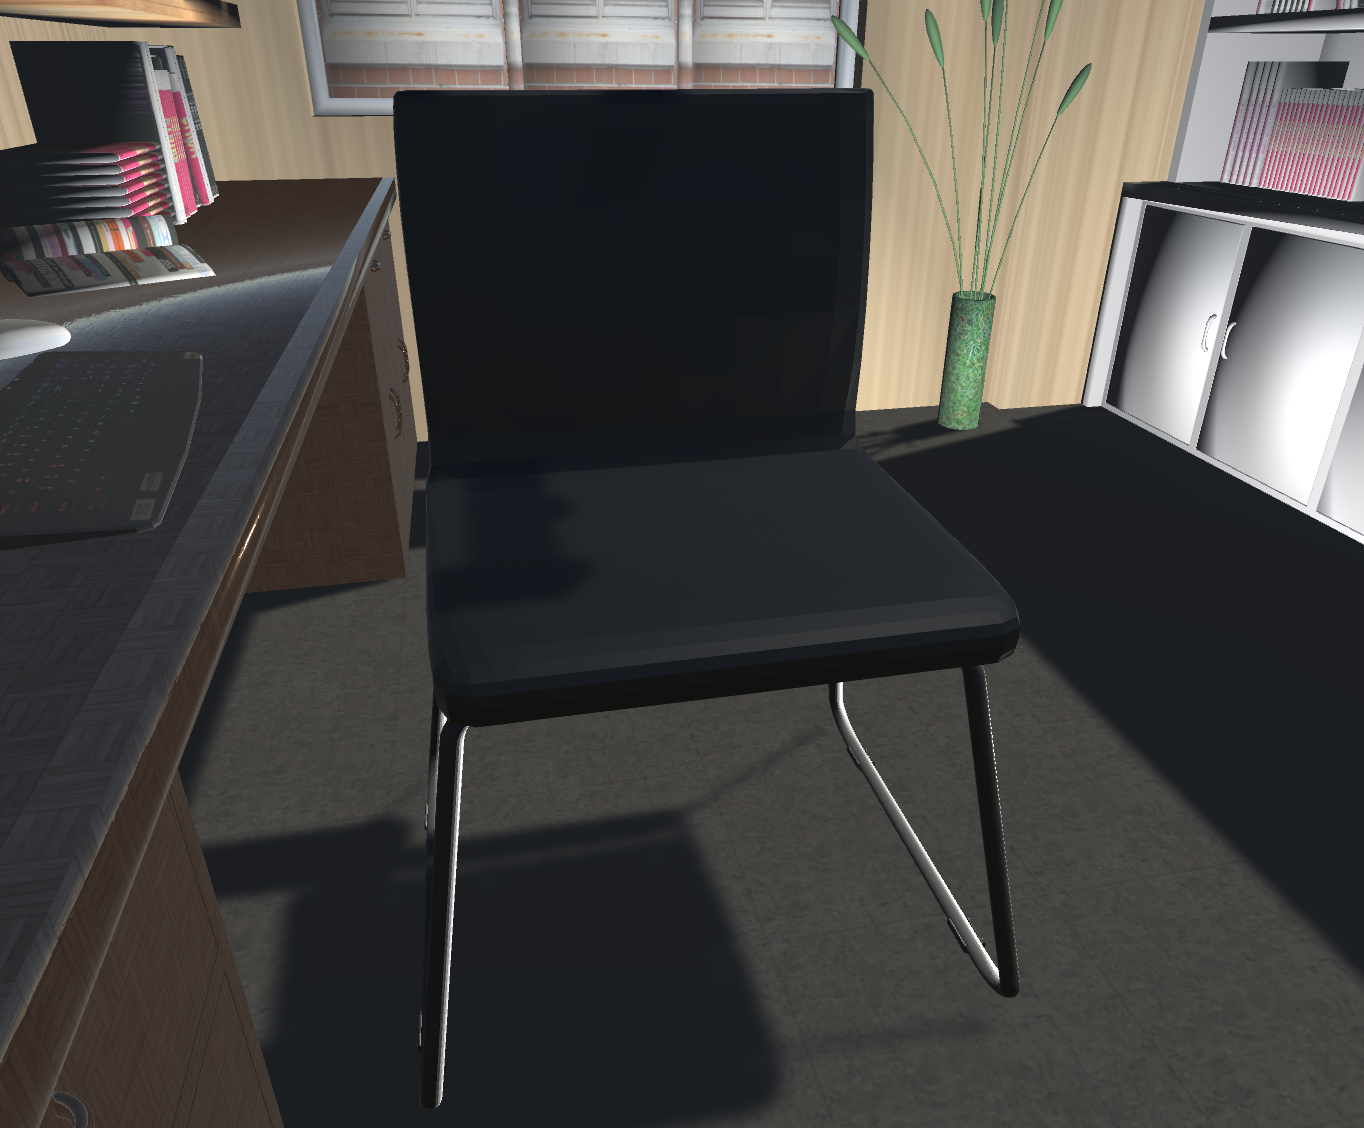
\includegraphics[width=.2\linewidth,valign=m]{/Users/apple/OVGU/Thesis/code/3dReconstruction/report/images/implementation/randomisation/camera1} &
        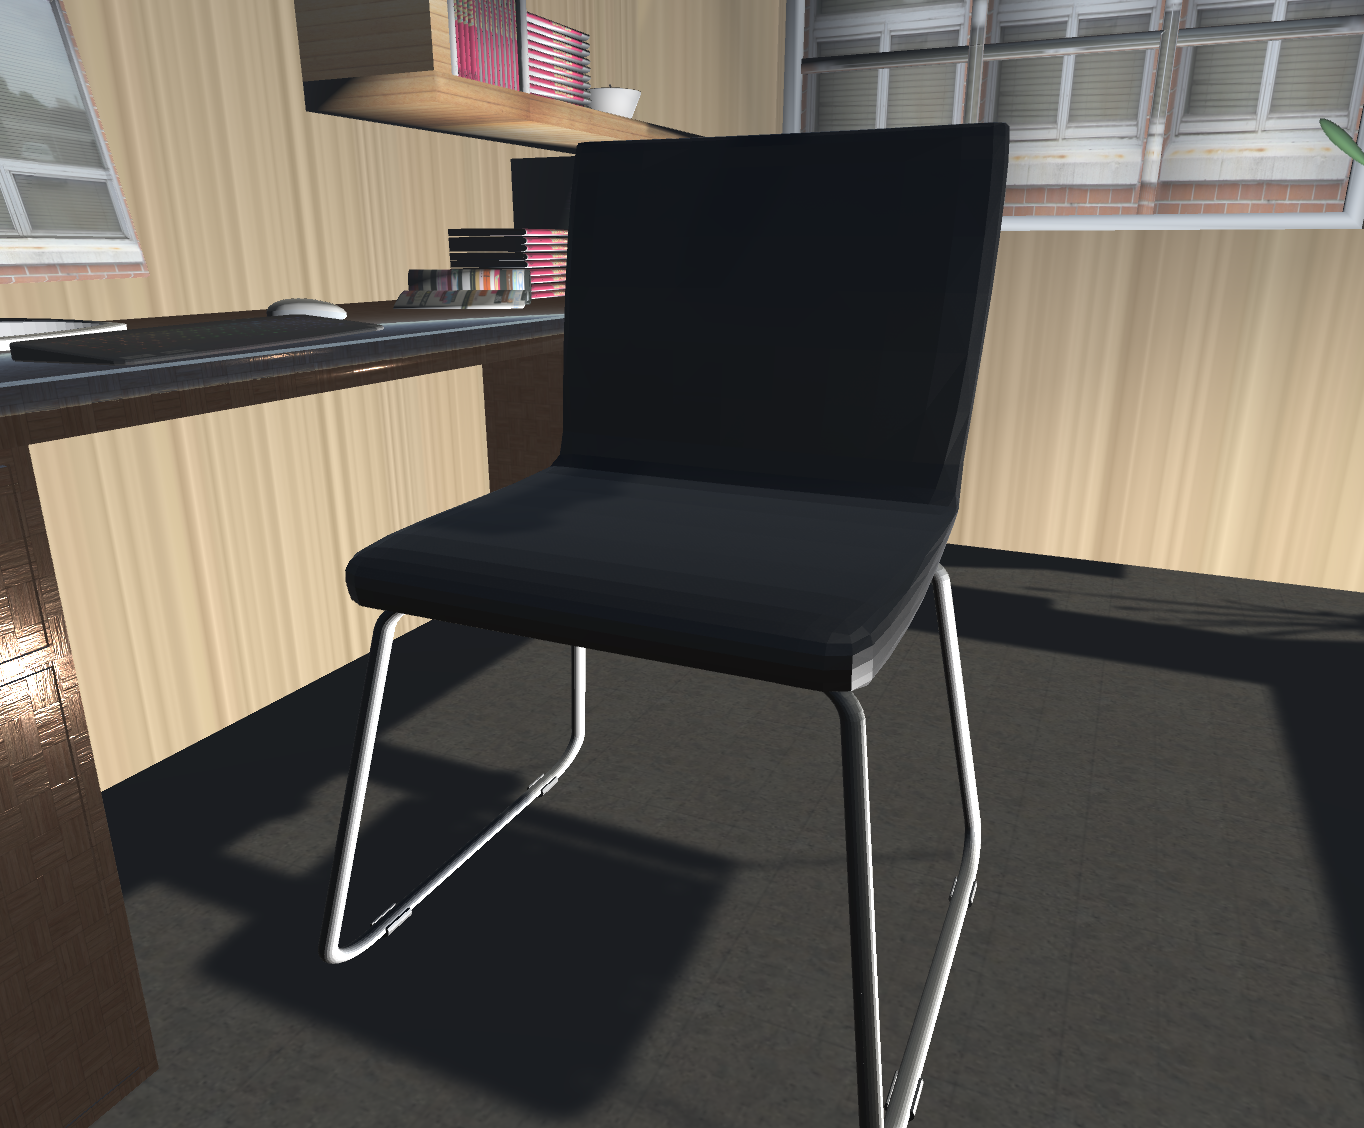
\includegraphics[width=.2\linewidth,valign=m]{/Users/apple/OVGU/Thesis/code/3dReconstruction/report/images/implementation/randomisation/camera2} &
        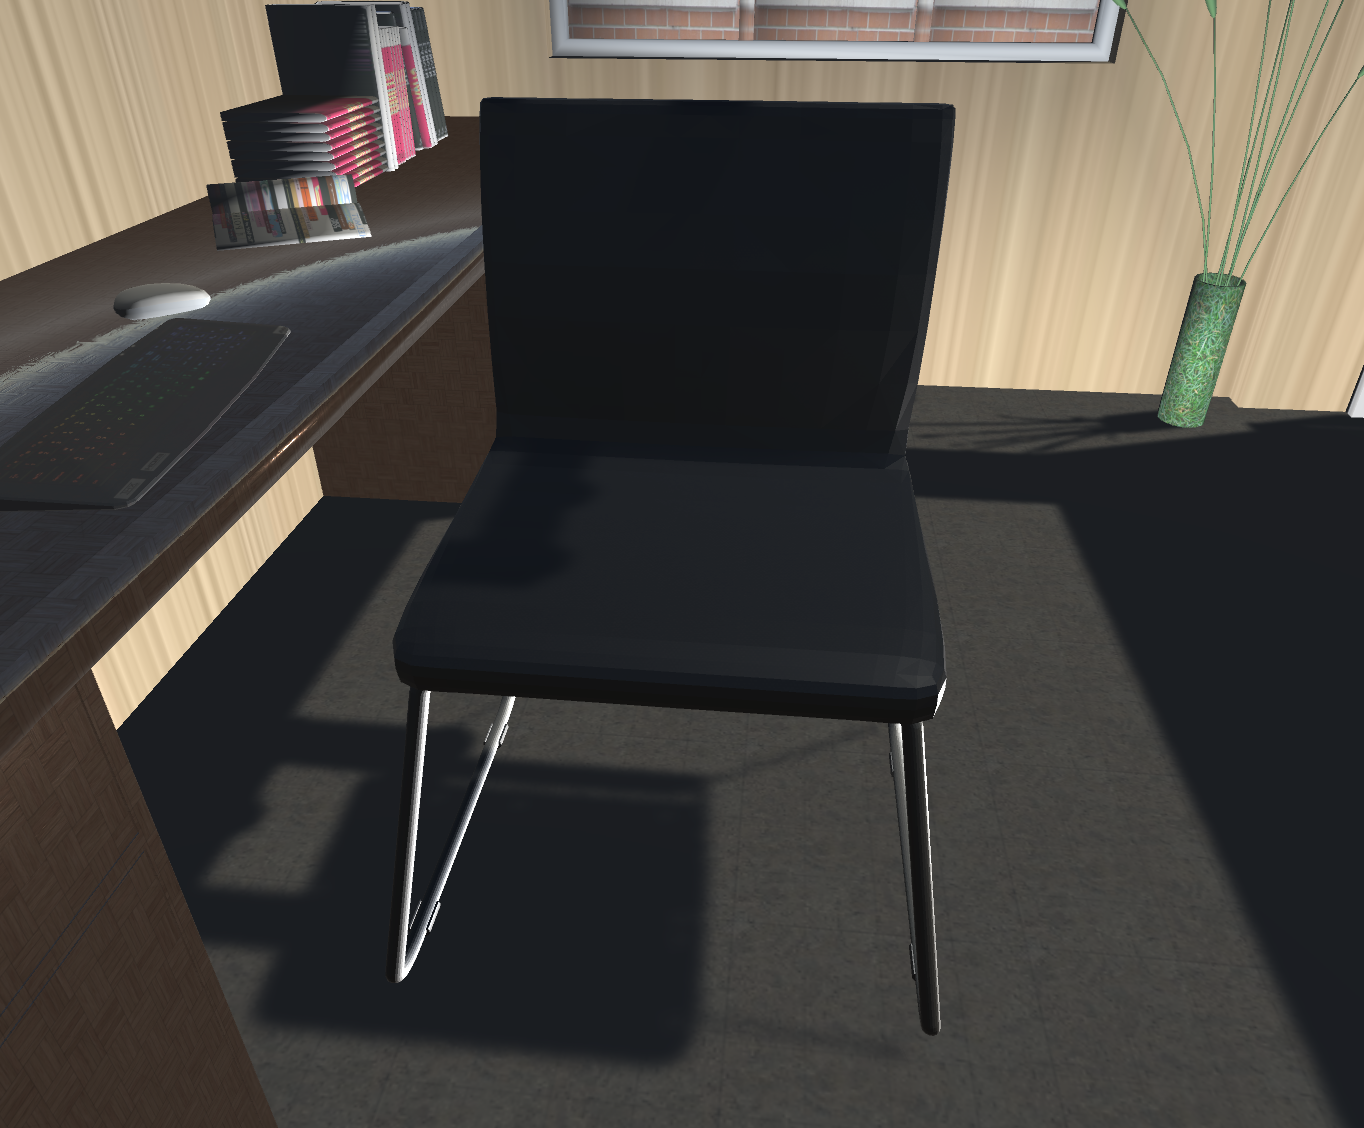
\includegraphics[width=.2\linewidth,valign=m]{/Users/apple/OVGU/Thesis/code/3dReconstruction/report/images/implementation/randomisation/camera3} &
        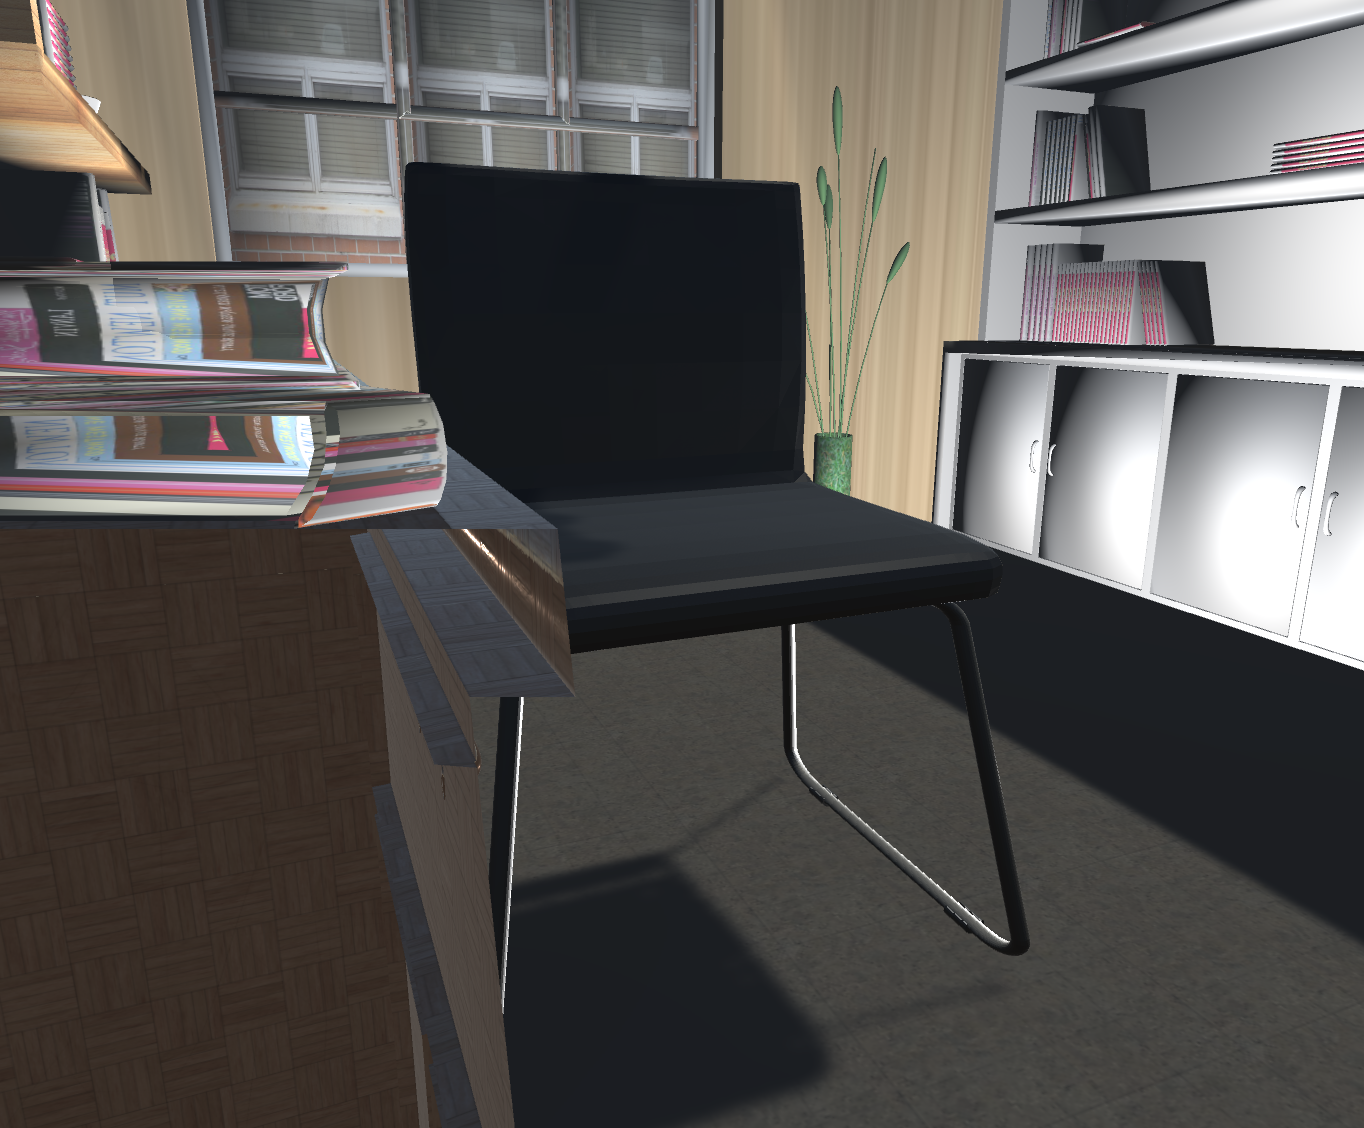
\includegraphics[width=.2\linewidth,valign=m]{/Users/apple/OVGU/Thesis/code/3dReconstruction/report/images/implementation/randomisation/camera4}\\
    \end{tabular}
    \caption{Sample images with different camera viewpoints of same object with a constant scene.}
    \label{fig:Camera viewpoints}
\end{figure}

\subsection{Lightings and Shadows}

We consider lighting to be a key component of the photorealism.
The shadows formed with different lighting condition enchance the photorealism of the images.
For this purpose we use 3 types of lights offered in Unity.

\begin{enumerate}
    \item Point light
    \item Spot light
    \item Sunlight
\end{enumerate}

Point lights act as indoor lights for the room the range of which can be varied.
We pre-define 6 light patterns for a room with cuboid shape.
Knowing the bounds of the room we decide how to place the lights by randomly select 1 to 6 lights with corresponding light patterns on the ceiling.
For the spotlight, only a single light is placed a meter above the target object.
This light gives a variation which focuses only on the target object.
Both point and spot-light have color variation along with varing brightness.
Sunlight is the default light settings in Unity.
This is specifically effective when the room has windows forming more realistic shadows.
In this case, we modulate the brightness and the angle at which the rays are emitted, which simulates different times of the day.

Another randomised entity is the skybox. Skybox acts as the outdoor scenes


\begin{figure}
    \begin{tabular}{llll}
        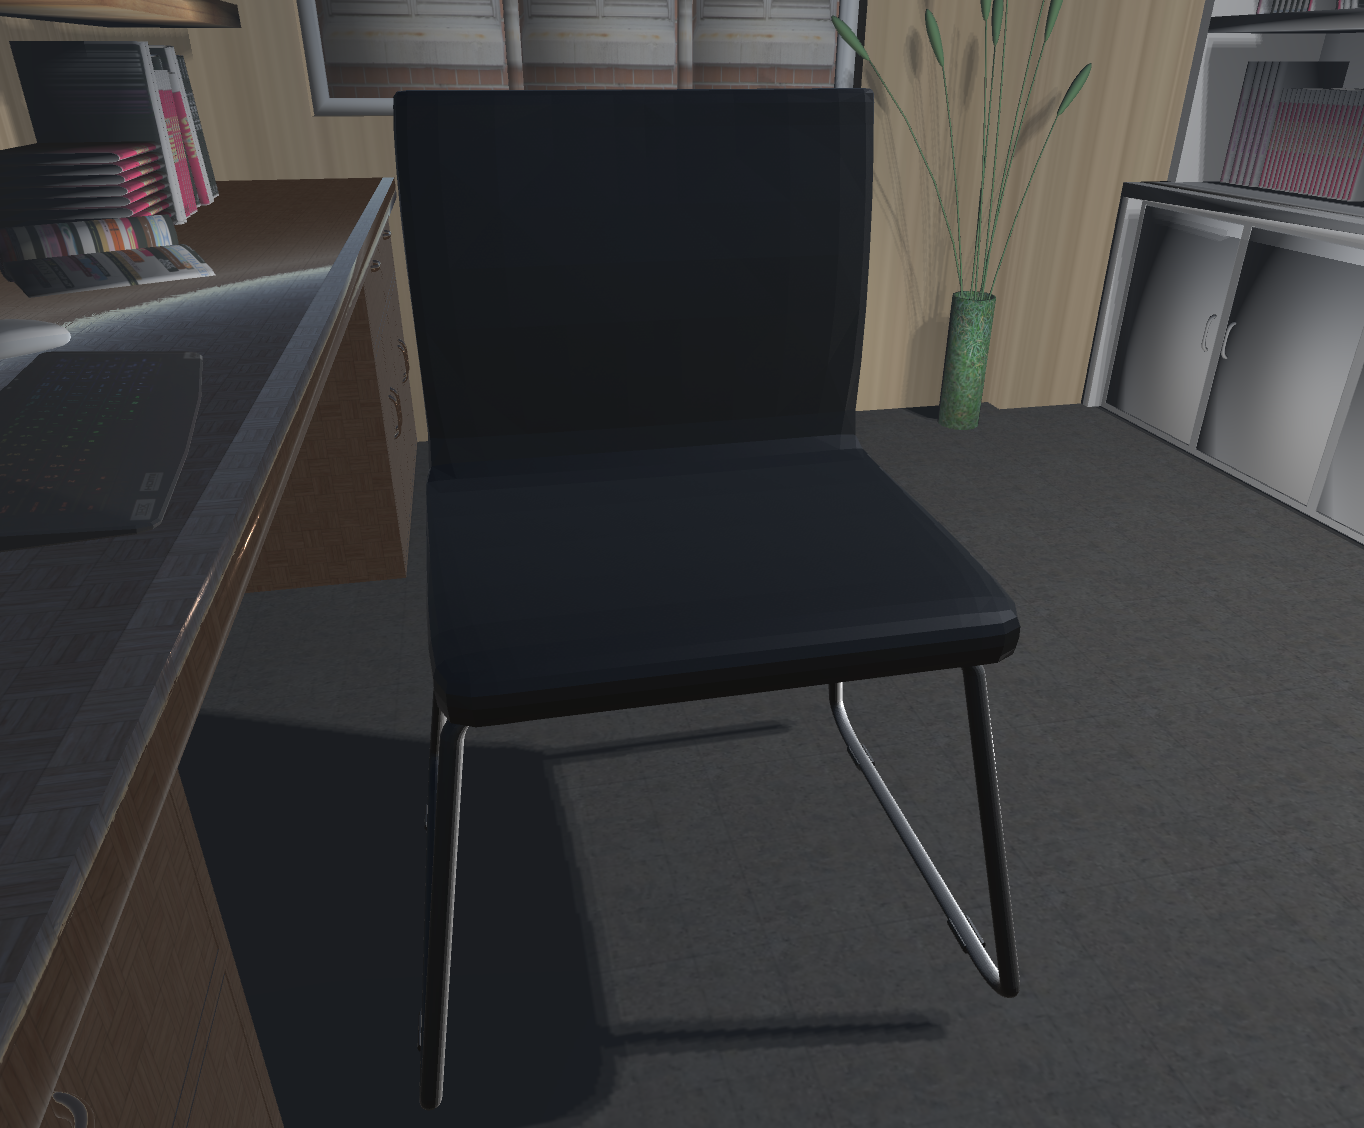
\includegraphics[width=.2\linewidth,valign=m]{/Users/apple/OVGU/Thesis/code/3dReconstruction/report/images/implementation/randomisation/lighting1} &
        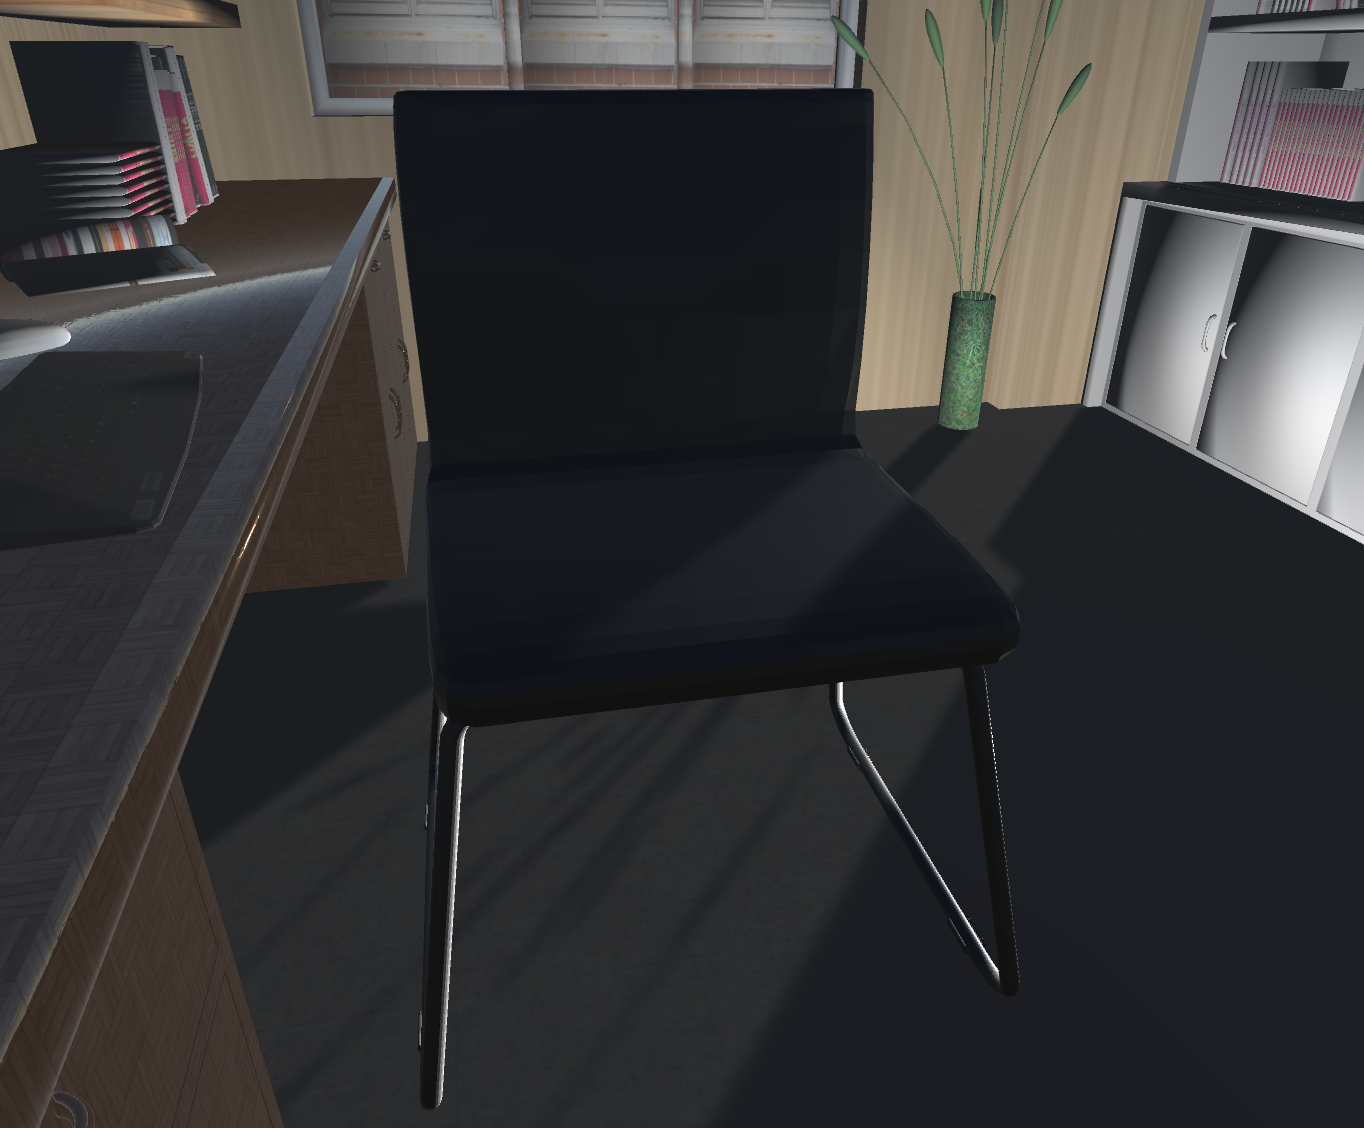
\includegraphics[width=.2\linewidth,valign=m]{/Users/apple/OVGU/Thesis/code/3dReconstruction/report/images/implementation/randomisation/lighting2} &
        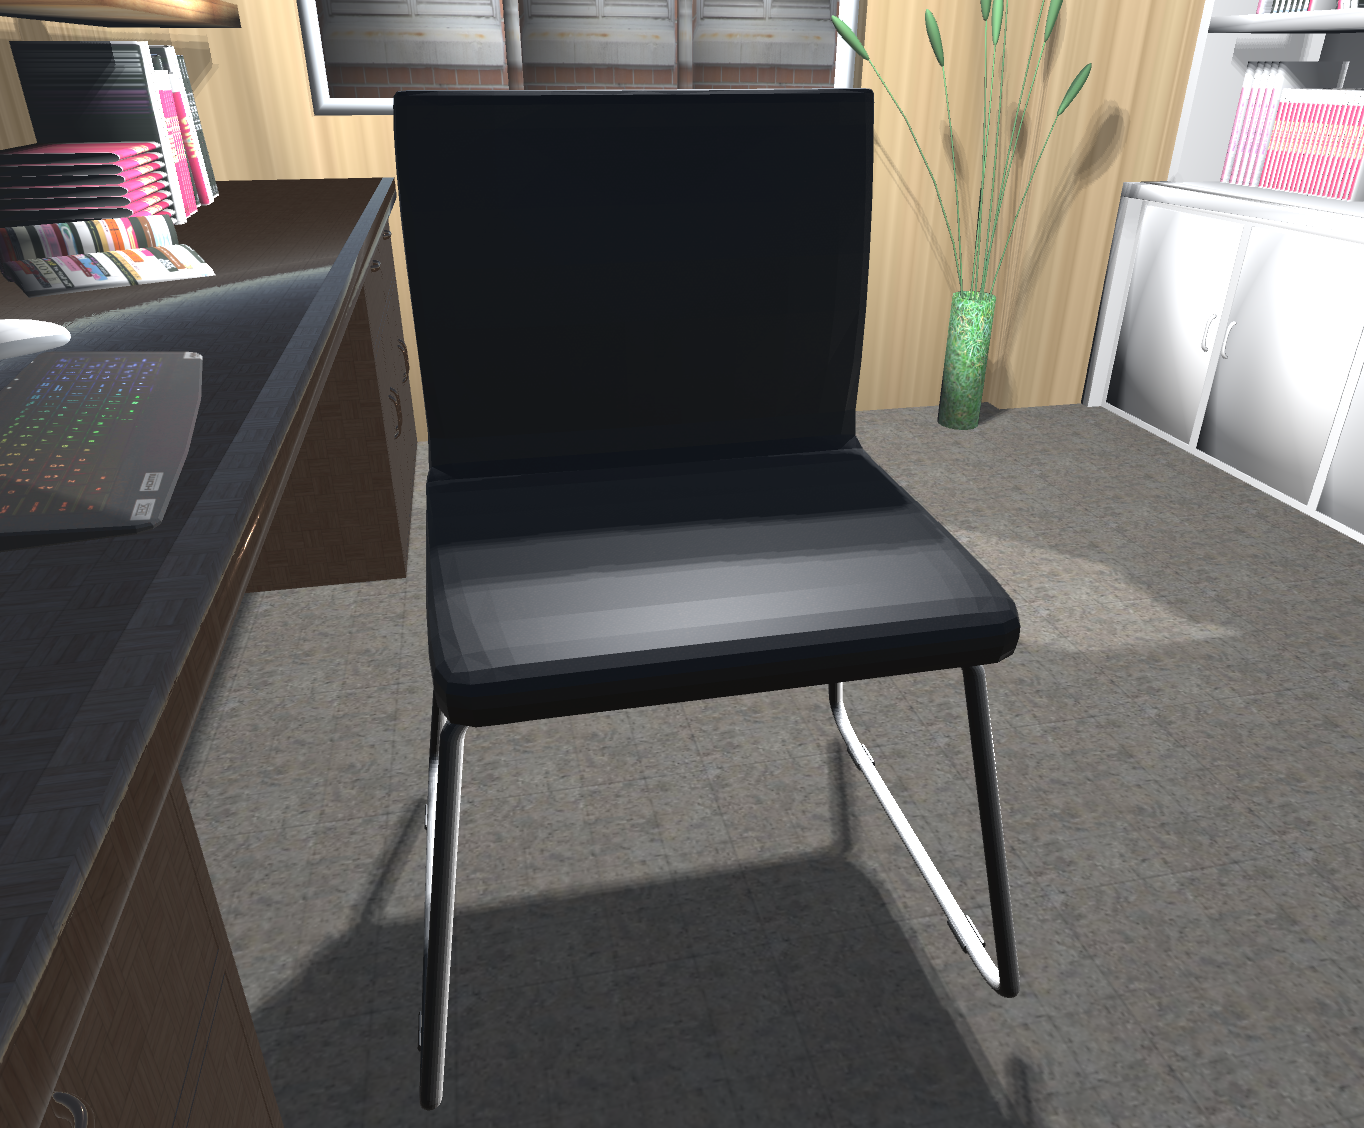
\includegraphics[width=.2\linewidth,valign=m]{/Users/apple/OVGU/Thesis/code/3dReconstruction/report/images/implementation/randomisation/lighting3} &
        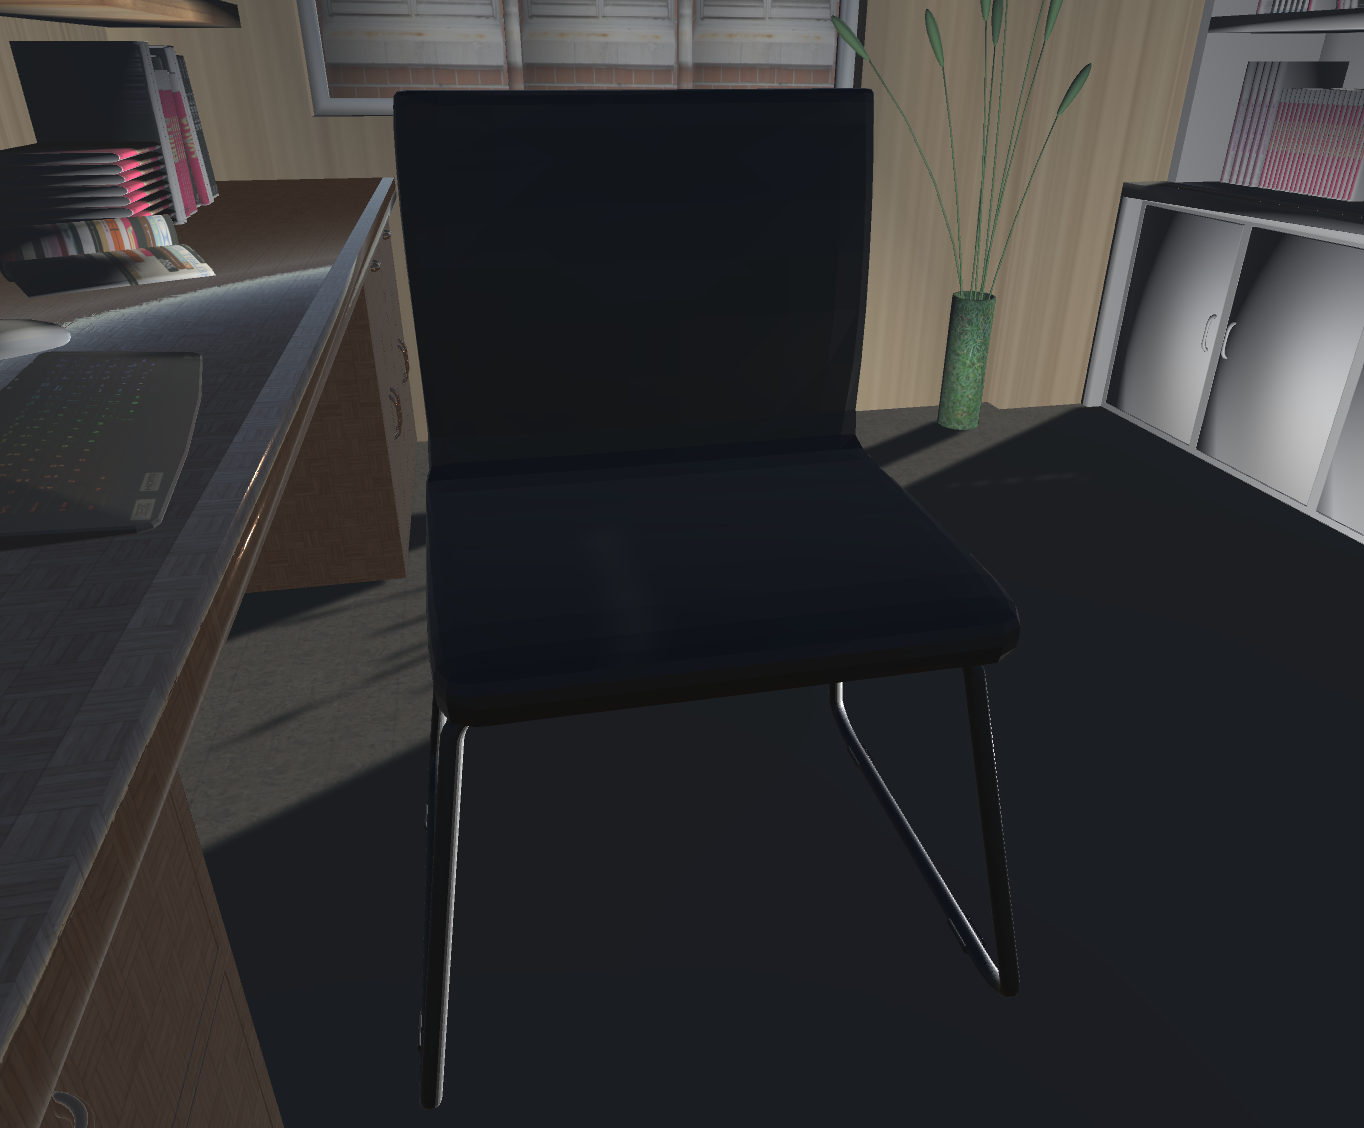
\includegraphics[width=.2\linewidth,valign=m]{/Users/apple/OVGU/Thesis/code/3dReconstruction/report/images/implementation/randomisation/lighting4}\\
    \end{tabular}
    \caption{Sample images with different lighting and shadows conditions}
    \label{fig:Lighting and shadows}
\end{figure}

\subsection{Randomised Texture}

\todo add distribution of textures from the folder

\begin{figure}
    \begin{tabular}{llll}
        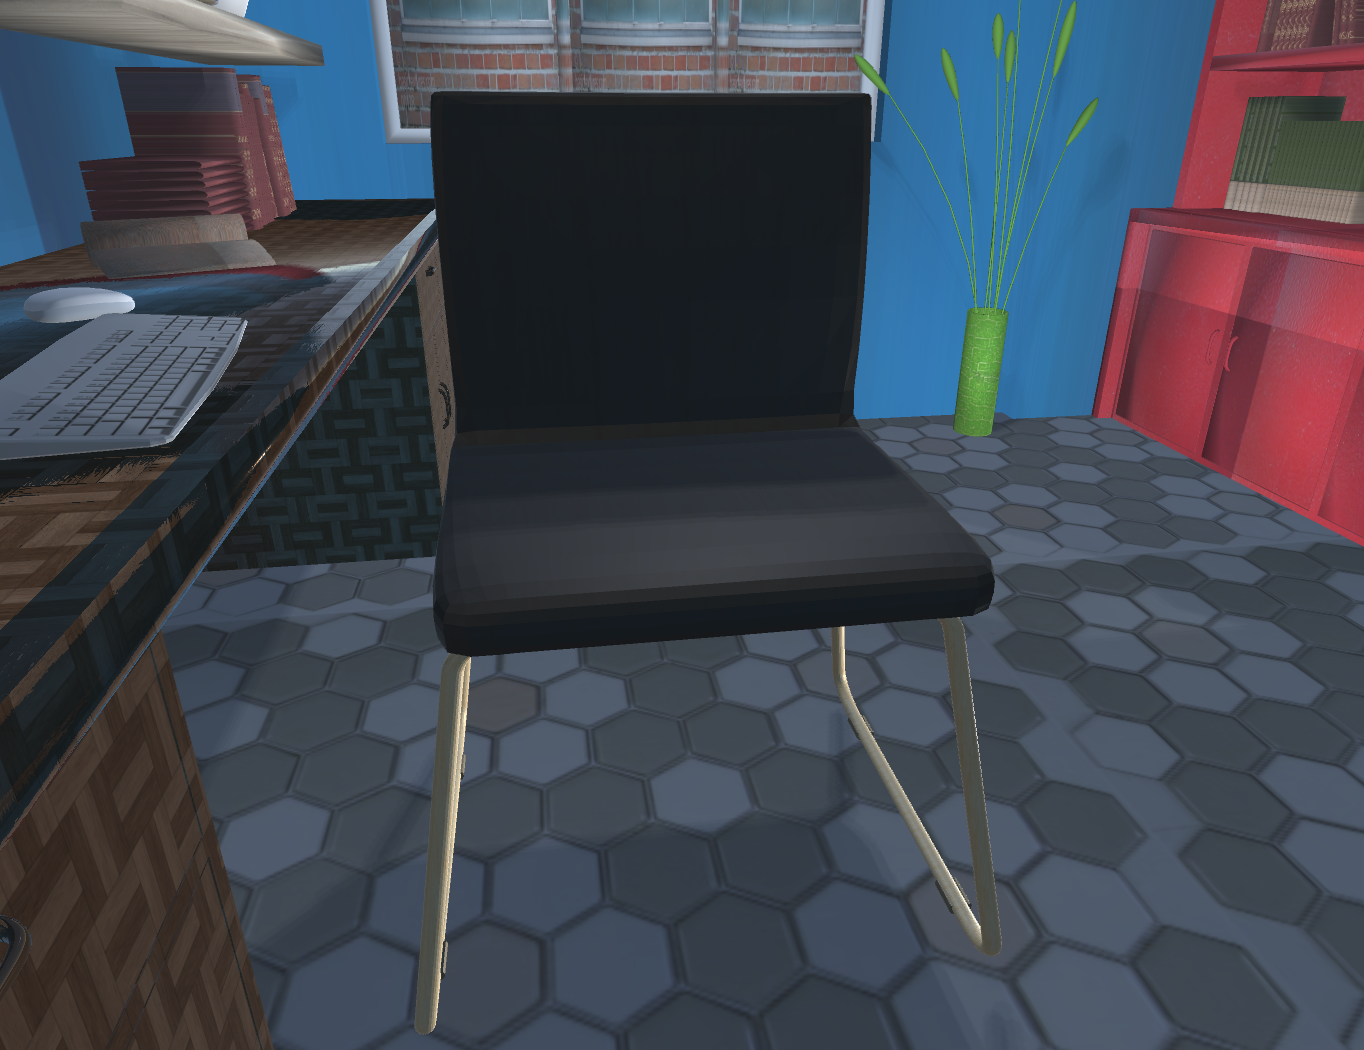
\includegraphics[width=.2\linewidth,valign=m]{/Users/apple/OVGU/Thesis/code/3dReconstruction/report/images/implementation/randomisation/background_texture1} &
        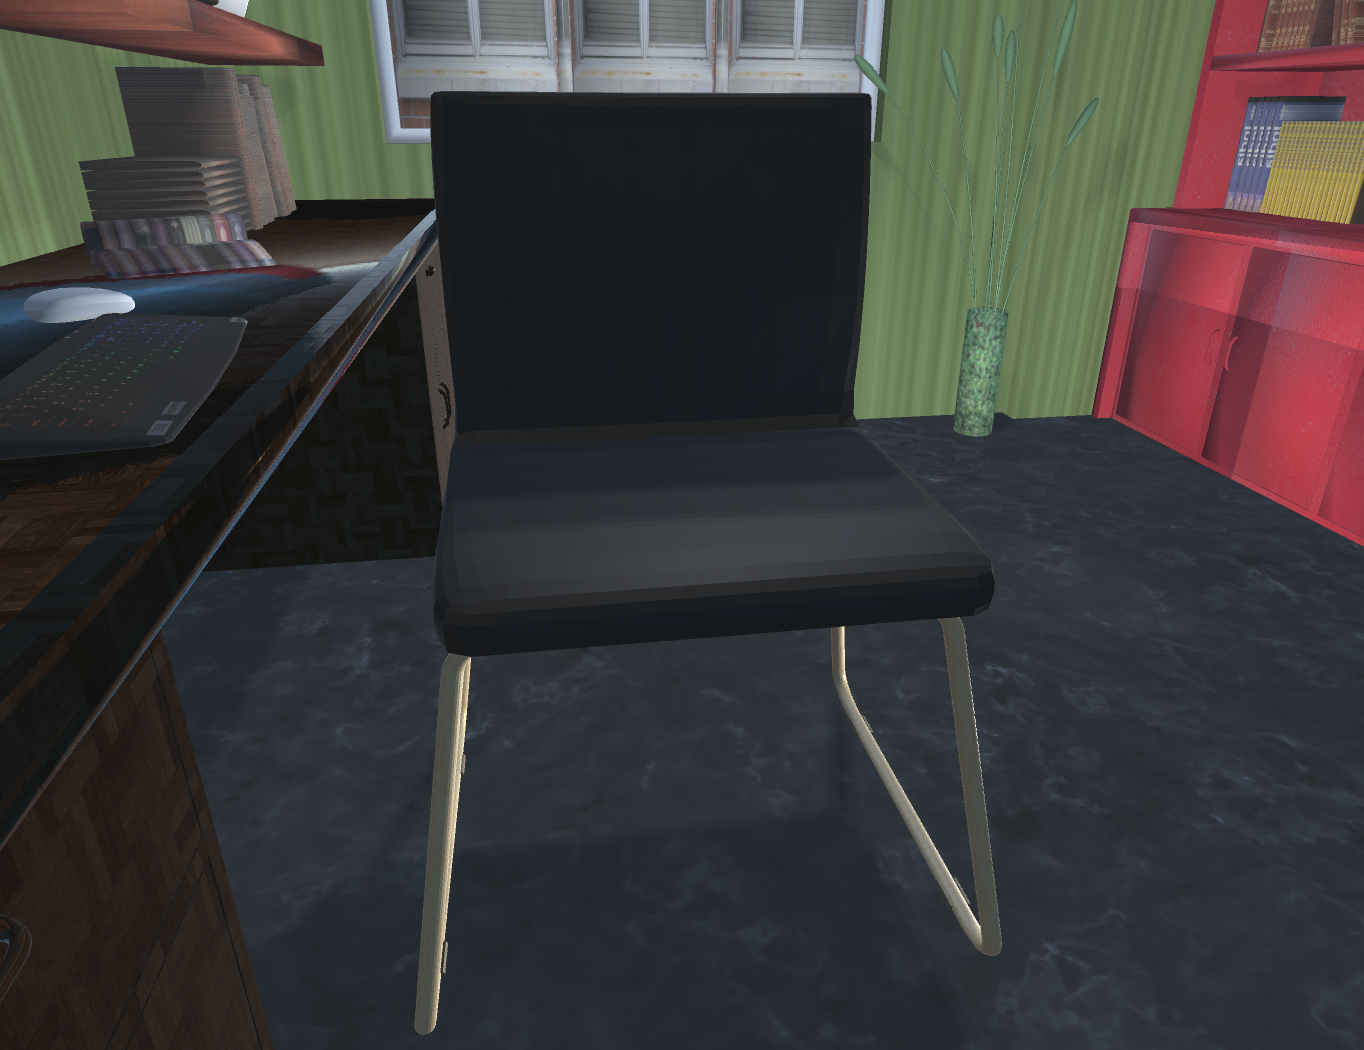
\includegraphics[width=.2\linewidth,valign=m]{/Users/apple/OVGU/Thesis/code/3dReconstruction/report/images/implementation/randomisation/background_texture2} &
        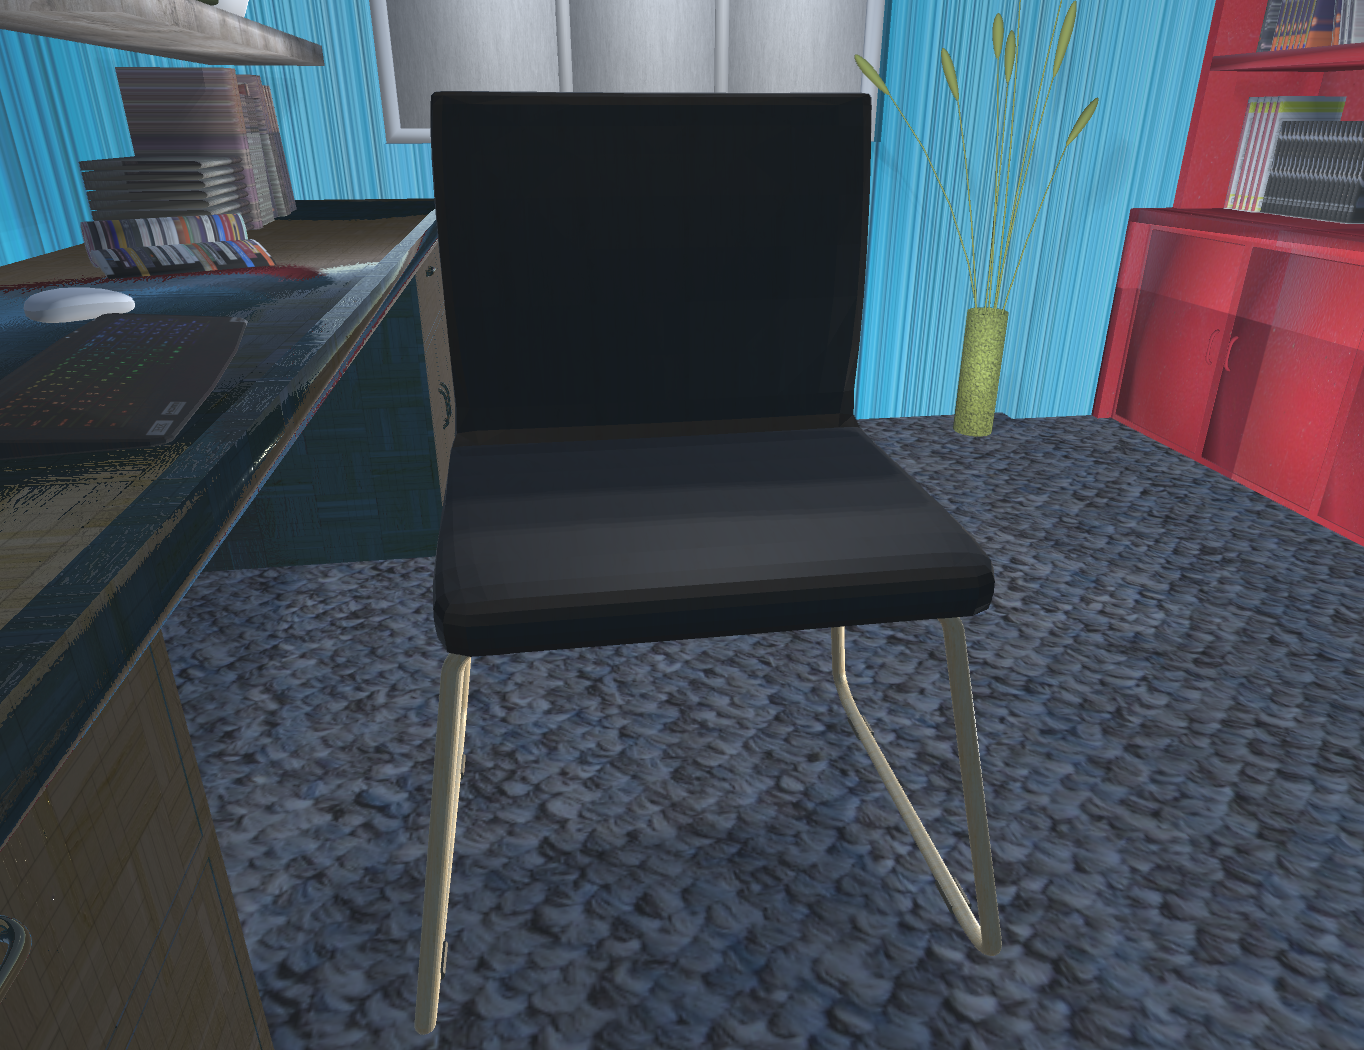
\includegraphics[width=.2\linewidth,valign=m]{/Users/apple/OVGU/Thesis/code/3dReconstruction/report/images/implementation/randomisation/background_texture3} &
        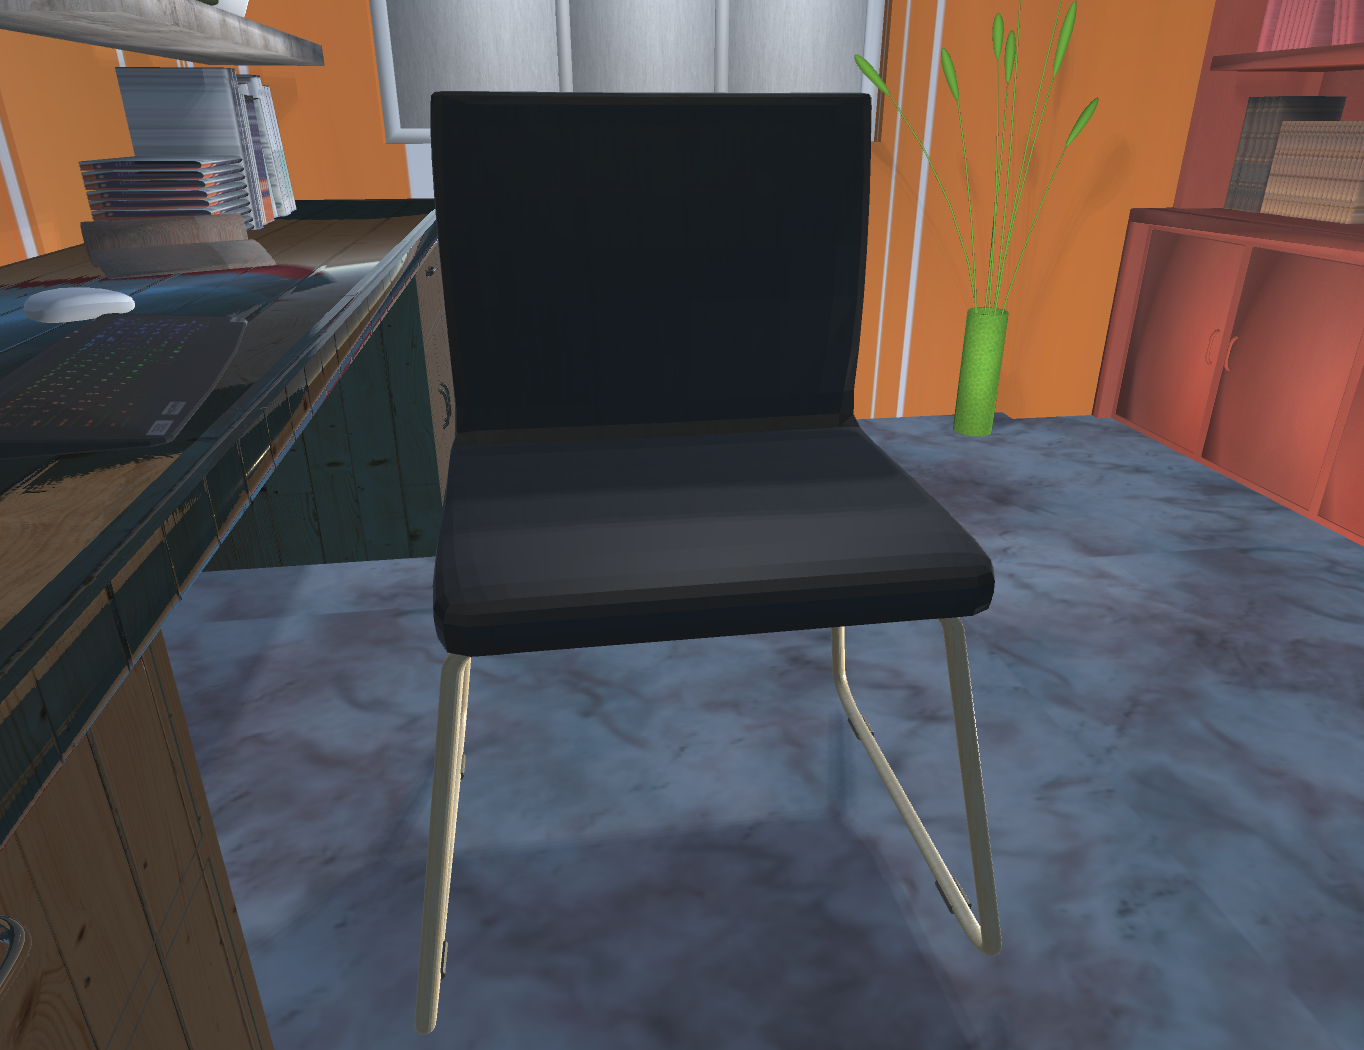
\includegraphics[width=.2\linewidth,valign=m]{/Users/apple/OVGU/Thesis/code/3dReconstruction/report/images/implementation/randomisation/background_texture4}\\
    \end{tabular}
    \caption{Sample images with different textures for same scene.}
    \label{fig:Texture Randomisation}
\end{figure}


\subsection{Replacing target Objects}

\begin{figure}
    \begin{tabular}{llll}
        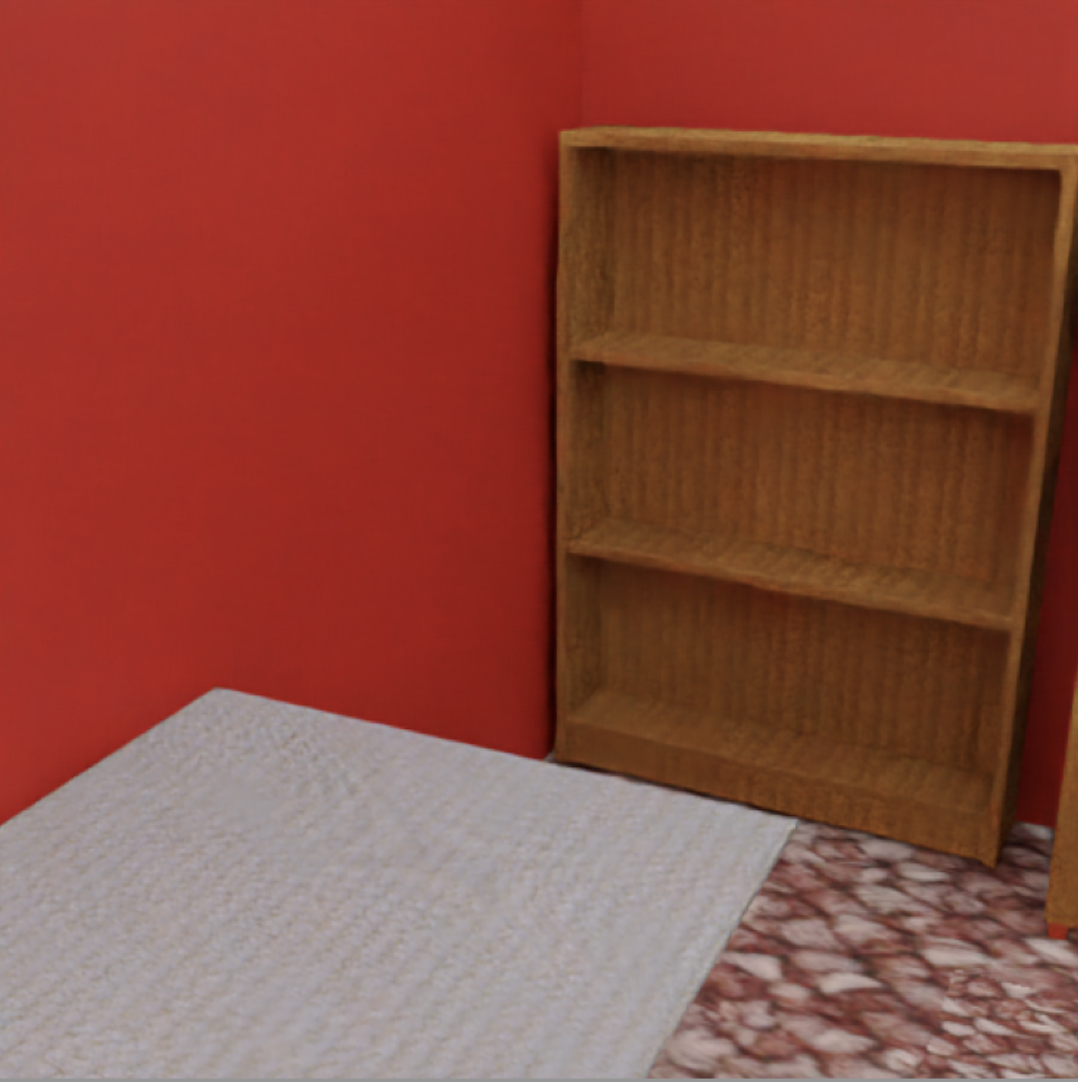
\includegraphics[width=.2\linewidth,valign=m]{/Users/apple/OVGU/Thesis/code/3dReconstruction/report/images/realistic_images_relatedwork/blenderproc_1} &
        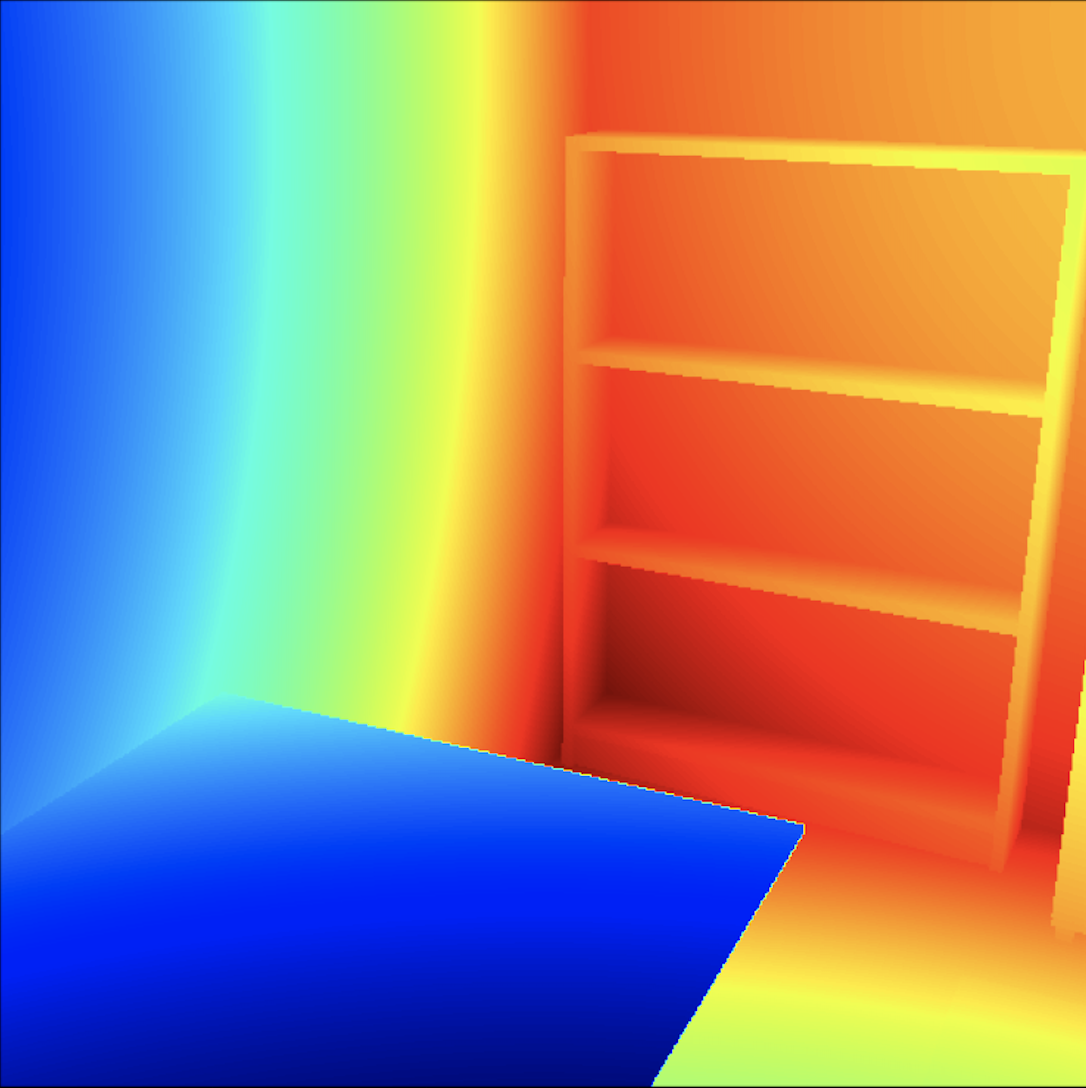
\includegraphics[width=.2\linewidth,valign=m]{/Users/apple/OVGU/Thesis/code/3dReconstruction/report/images/realistic_images_relatedwork/blenderproc_depth_1} &
        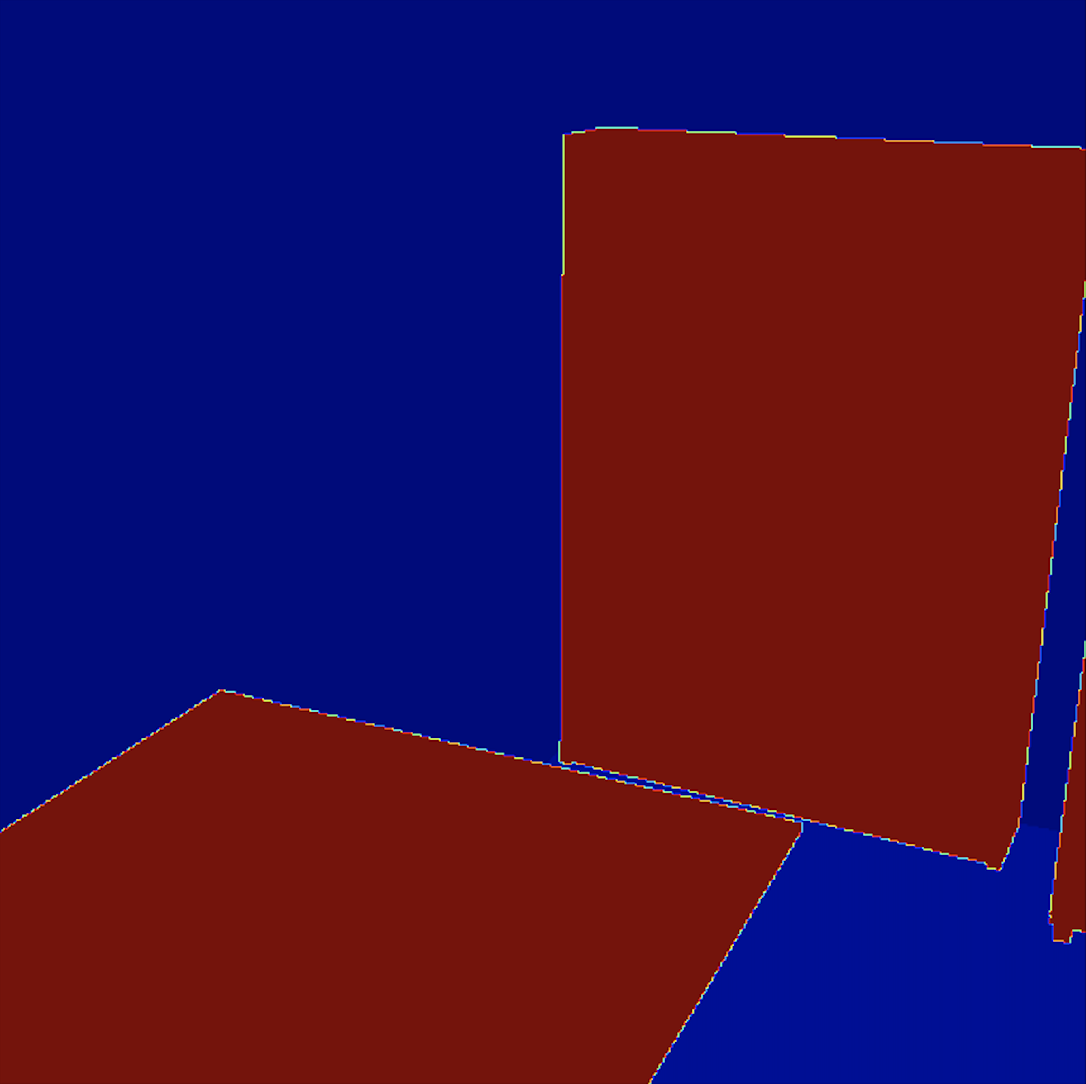
\includegraphics[width=.2\linewidth,valign=m]{/Users/apple/OVGU/Thesis/code/3dReconstruction/report/images/realistic_images_relatedwork/blenderproc_instance_1} &
        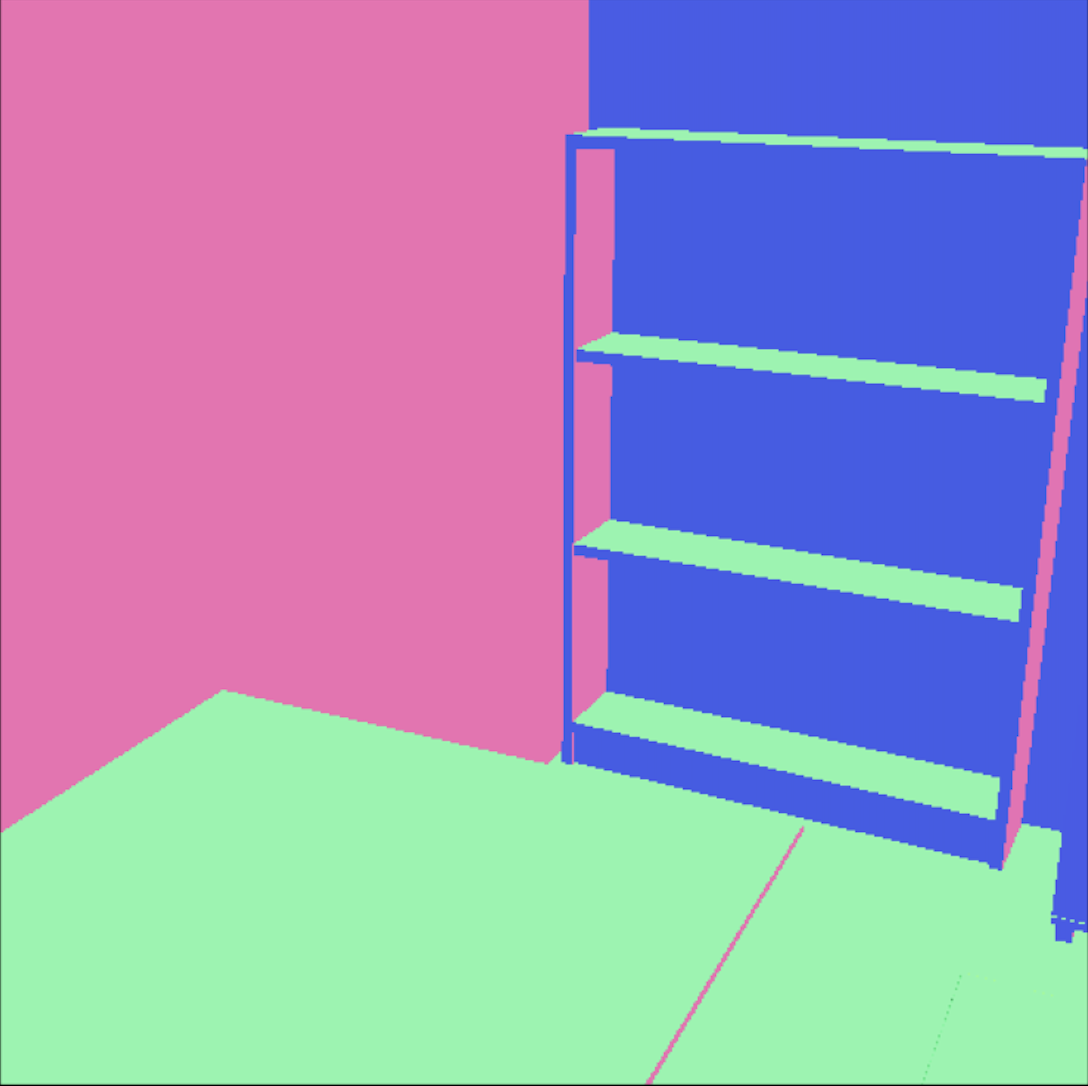
\includegraphics[width=.2\linewidth,valign=m]{/Users/apple/OVGU/Thesis/code/3dReconstruction/report/images/realistic_images_relatedwork/blenderproc_normal_1}\\
    \end{tabular}
    \caption{Sample images created from BlenderProc using SceneNet dataset.(Left to right) RGB images, Depth Maps, Instance Segmenatations and Normals. Each row is an independent sample.}
    \label{fig:Replacing target objects}
\end{figure}

Replacing models, lighting(indoor and outdoor), randomisation of texture, camera distance, camera angles, outdoor skybox,
UI controls
Manual inputs, automated
Unity - ML-ImageSynthesis
UML diagram is needed? (If it helps)

\section{3d-Reconstruction framework}
Development environment
Training setup(hardware, voxel size…)
Mixed precision using apex
If mixed precision helped performance, memory, speed, evaluation metric


\section{Implement a domain adaptation technique}
To serve as a proof if more domain gap reduction is needed
